\documentclass[1p]{elsarticle_modified}
%\bibliographystyle{elsarticle-num}

%\usepackage[colorlinks]{hyperref}
%\usepackage{abbrmath_seonhwa} %\Abb, \Ascr, \Acal ,\Abf, \Afrak
\usepackage{amsfonts}
\usepackage{amssymb}
\usepackage{amsmath}
\usepackage{amsthm}
\usepackage{scalefnt}
\usepackage{amsbsy}
\usepackage{kotex}
\usepackage{caption}
\usepackage{subfig}
\usepackage{color}
\usepackage{graphicx}
\usepackage{xcolor} %% white, black, red, green, blue, cyan, magenta, yellow
\usepackage{float}
\usepackage{setspace}
\usepackage{hyperref}

\usepackage{tikz}
\usetikzlibrary{arrows}

\usepackage{multirow}
\usepackage{array} % fixed length table
\usepackage{hhline}

%%%%%%%%%%%%%%%%%%%%%
\makeatletter
\renewcommand*\env@matrix[1][\arraystretch]{%
	\edef\arraystretch{#1}%
	\hskip -\arraycolsep
	\let\@ifnextchar\new@ifnextchar
	\array{*\c@MaxMatrixCols c}}
\makeatother %https://tex.stackexchange.com/questions/14071/how-can-i-increase-the-line-spacing-in-a-matrix
%%%%%%%%%%%%%%%

\usepackage[normalem]{ulem}

\newcommand{\msout}[1]{\ifmmode\text{\sout{\ensuremath{#1}}}\else\sout{#1}\fi}
%SOURCE: \msout is \stkout macro in https://tex.stackexchange.com/questions/20609/strikeout-in-math-mode

\newcommand{\cancel}[1]{
	\ifmmode
	{\color{red}\msout{#1}}
	\else
	{\color{red}\sout{#1}}
	\fi
}

\newcommand{\add}[1]{
	{\color{blue}\uwave{#1}}
}

\newcommand{\replace}[2]{
	\ifmmode
	{\color{red}\msout{#1}}{\color{blue}\uwave{#2}}
	\else
	{\color{red}\sout{#1}}{\color{blue}\uwave{#2}}
	\fi
}

\newcommand{\Sol}{\mathcal{S}} %segment
\newcommand{\D}{D} %diagram
\newcommand{\A}{\mathcal{A}} %arc


%%%%%%%%%%%%%%%%%%%%%%%%%%%%%5 test

\def\sl{\operatorname{\textup{SL}}(2,\Cbb)}
\def\psl{\operatorname{\textup{PSL}}(2,\Cbb)}
\def\quan{\mkern 1mu \triangleright \mkern 1mu}

\theoremstyle{definition}
\newtheorem{thm}{Theorem}[section]
\newtheorem{prop}[thm]{Proposition}
\newtheorem{lem}[thm]{Lemma}
\newtheorem{ques}[thm]{Question}
\newtheorem{cor}[thm]{Corollary}
\newtheorem{defn}[thm]{Definition}
\newtheorem{exam}[thm]{Example}
\newtheorem{rmk}[thm]{Remark}
\newtheorem{alg}[thm]{Algorithm}

\newcommand{\I}{\sqrt{-1}}
\begin{document}

%\begin{frontmatter}
%
%\title{Boundary parabolic representations of knots up to 8 crossings}
%
%%% Group authors per affiliation:
%\author{Yunhi Cho} 
%\address{Department of Mathematics, University of Seoul, Seoul, Korea}
%\ead{yhcho@uos.ac.kr}
%
%
%\author{Seonhwa Kim} %\fnref{s_kim}}
%\address{Center for Geometry and Physics, Institute for Basic Science, Pohang, 37673, Korea}
%\ead{ryeona17@ibs.re.kr}
%
%\author{Hyuk Kim}
%\address{Department of Mathematical Sciences, Seoul National University, Seoul 08826, Korea}
%\ead{hyukkim@snu.ac.kr}
%
%\author{Seokbeom Yoon}
%\address{Department of Mathematical Sciences, Seoul National University, Seoul, 08826,  Korea}
%\ead{sbyoon15@snu.ac.kr}
%
%\begin{abstract}
%We find all boundary parabolic representation of knots up to 8 crossings.
%
%\end{abstract}
%\begin{keyword}
%    \MSC[2010] 57M25 
%\end{keyword}
%
%\end{frontmatter}

%\linenumbers
%\tableofcontents
%
\newcommand\colored[1]{\textcolor{white}{\rule[-0.35ex]{0.8em}{1.4ex}}\kern-0.8em\color{red} #1}%
%\newcommand\colored[1]{\textcolor{white}{ #1}\kern-2.17ex	\textcolor{white}{ #1}\kern-1.81ex	\textcolor{white}{ #1}\kern-2.15ex\color{red}#1	}

{\Large $\underline{12n_{0390}~(K12n_{0390})}$}

\setlength{\tabcolsep}{10pt}
\renewcommand{\arraystretch}{1.6}
\vspace{1cm}\begin{tabular}{m{100pt}>{\centering\arraybackslash}m{274pt}}
\multirow{5}{120pt}{
	\centering
	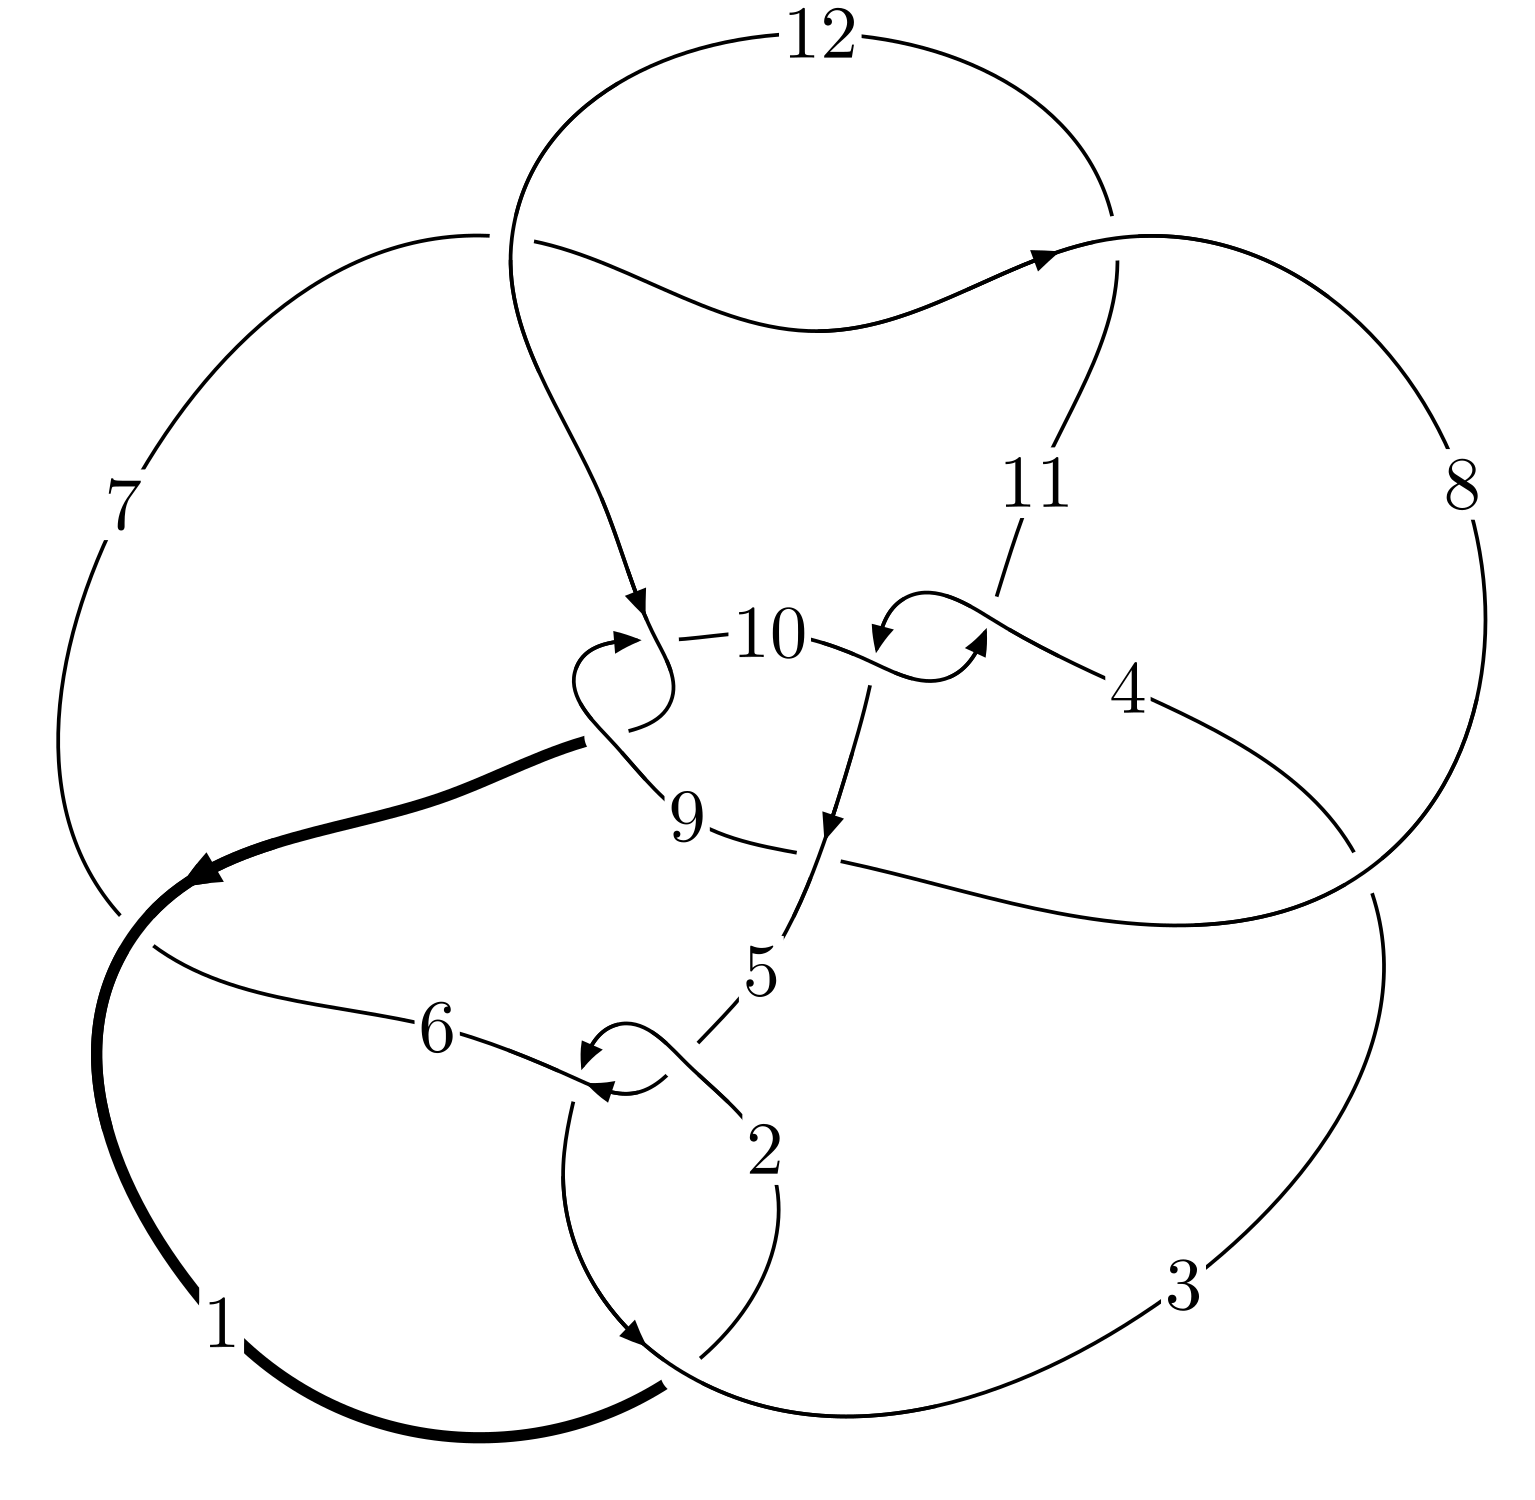
\includegraphics[width=112pt]{../../../GIT/diagram.site/Diagrams/png/2479_12n_0390.png}\\
\ \ \ A knot diagram\footnotemark}&
\allowdisplaybreaks
\textbf{Linearized knot diagam} \\
\cline{2-2}
 &
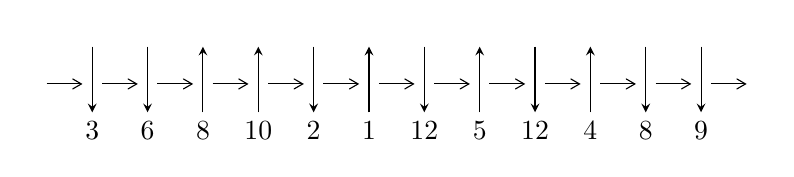
\begin{tikzpicture}[x=20pt, y=17pt]
	% nodes
	\node (C0) at (0, 0) {};
	\node (C1) at (1, 0) {};
	\node (C1U) at (1, +1) {};
	\node (C1D) at (1, -1) {3};

	\node (C2) at (2, 0) {};
	\node (C2U) at (2, +1) {};
	\node (C2D) at (2, -1) {6};

	\node (C3) at (3, 0) {};
	\node (C3U) at (3, +1) {};
	\node (C3D) at (3, -1) {8};

	\node (C4) at (4, 0) {};
	\node (C4U) at (4, +1) {};
	\node (C4D) at (4, -1) {10};

	\node (C5) at (5, 0) {};
	\node (C5U) at (5, +1) {};
	\node (C5D) at (5, -1) {2};

	\node (C6) at (6, 0) {};
	\node (C6U) at (6, +1) {};
	\node (C6D) at (6, -1) {1};

	\node (C7) at (7, 0) {};
	\node (C7U) at (7, +1) {};
	\node (C7D) at (7, -1) {12};

	\node (C8) at (8, 0) {};
	\node (C8U) at (8, +1) {};
	\node (C8D) at (8, -1) {5};

	\node (C9) at (9, 0) {};
	\node (C9U) at (9, +1) {};
	\node (C9D) at (9, -1) {12};

	\node (C10) at (10, 0) {};
	\node (C10U) at (10, +1) {};
	\node (C10D) at (10, -1) {4};

	\node (C11) at (11, 0) {};
	\node (C11U) at (11, +1) {};
	\node (C11D) at (11, -1) {8};

	\node (C12) at (12, 0) {};
	\node (C12U) at (12, +1) {};
	\node (C12D) at (12, -1) {9};
	\node (C13) at (13, 0) {};

	% arrows
	\draw[->,>={angle 60}]
	(C0) edge (C1) (C1) edge (C2) (C2) edge (C3) (C3) edge (C4) (C4) edge (C5) (C5) edge (C6) (C6) edge (C7) (C7) edge (C8) (C8) edge (C9) (C9) edge (C10) (C10) edge (C11) (C11) edge (C12) (C12) edge (C13) ;	\draw[->,>=stealth]
	(C1U) edge (C1D) (C2U) edge (C2D) (C3D) edge (C3U) (C4D) edge (C4U) (C5U) edge (C5D) (C6D) edge (C6U) (C7U) edge (C7D) (C8D) edge (C8U) (C9U) edge (C9D) (C10D) edge (C10U) (C11U) edge (C11D) (C12U) edge (C12D) ;
	\end{tikzpicture} \\
\hhline{~~} \\& 
\textbf{Solving Sequence} \\ \cline{2-2} 
 &
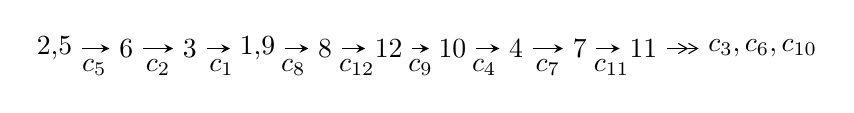
\begin{tikzpicture}[x=23pt, y=7pt]
	% node
	\node (A0) at (-1/8, 0) {2,5};
	\node (A1) at (1, 0) {6};
	\node (A2) at (2, 0) {3};
	\node (A3) at (49/16, 0) {1,9};
	\node (A4) at (33/8, 0) {8};
	\node (A5) at (41/8, 0) {12};
	\node (A6) at (49/8, 0) {10};
	\node (A7) at (57/8, 0) {4};
	\node (A8) at (65/8, 0) {7};
	\node (A9) at (73/8, 0) {11};
	\node (C1) at (1/2, -1) {$c_{5}$};
	\node (C2) at (3/2, -1) {$c_{2}$};
	\node (C3) at (5/2, -1) {$c_{1}$};
	\node (C4) at (29/8, -1) {$c_{8}$};
	\node (C5) at (37/8, -1) {$c_{12}$};
	\node (C6) at (45/8, -1) {$c_{9}$};
	\node (C7) at (53/8, -1) {$c_{4}$};
	\node (C8) at (61/8, -1) {$c_{7}$};
	\node (C9) at (69/8, -1) {$c_{11}$};
	\node (A10) at (11, 0) {$c_{3},c_{6},c_{10}$};

	% edge
	\draw[->,>=stealth]	
	(A0) edge (A1) (A1) edge (A2) (A2) edge (A3) (A3) edge (A4) (A4) edge (A5) (A5) edge (A6) (A6) edge (A7) (A7) edge (A8) (A8) edge (A9) ;
	\draw[->>,>={angle 60}]	
	(A9) edge (A10);
\end{tikzpicture} \\ 

\end{tabular} \\

\footnotetext{
The image of knot diagram is generated by the software ``\textbf{Draw programme}" developed by Andrew Bartholomew(\url{http://www.layer8.co.uk/maths/draw/index.htm\#Running-draw}), where we modified some parts for our purpose(\url{https://github.com/CATsTAILs/LinksPainter}).
}\phantom \\ \newline 
\centering \textbf{Ideals for irreducible components\footnotemark of $X_{\text{par}}$} 
 
\begin{align*}
I^u_{1}&=\langle 
2.46294\times10^{29} u^{46}+7.95784\times10^{29} u^{45}+\cdots+2.37042\times10^{29} b-6.34182\times10^{30},\\
\phantom{I^u_{1}}&\phantom{= \langle  }1.94482\times10^{31} u^{46}+4.33728\times10^{31} u^{45}+\cdots+2.60747\times10^{30} a-2.49401\times10^{32},\;u^{47}+3 u^{46}+\cdots-40 u-11\rangle \\
I^u_{2}&=\langle 
- u^{15}- u^{14}+4 u^{13}+4 u^{12}-9 u^{11}-8 u^{10}+12 u^9+6 u^8-11 u^7+2 u^6+6 u^5-7 u^4-2 u^3+3 u^2+b,\\
\phantom{I^u_{2}}&\phantom{= \langle  }-2 u^{17}-3 u^{16}+\cdots+a+2,\;u^{18}-5 u^{16}+\cdots- u+1\rangle \\
\\
\end{align*}
\raggedright * 2 irreducible components of $\dim_{\mathbb{C}}=0$, with total 65 representations.\\
\footnotetext{All coefficients of polynomials are rational numbers. But the coefficients are sometimes approximated in decimal forms when there is not enough margin.}
\newpage
\renewcommand{\arraystretch}{1}
\centering \section*{I. $I^u_{1}= \langle 2.46\times10^{29} u^{46}+7.96\times10^{29} u^{45}+\cdots+2.37\times10^{29} b-6.34\times10^{30},\;1.94\times10^{31} u^{46}+4.34\times10^{31} u^{45}+\cdots+2.61\times10^{30} a-2.49\times10^{32},\;u^{47}+3 u^{46}+\cdots-40 u-11 \rangle$}
\flushleft \textbf{(i) Arc colorings}\\
\begin{tabular}{m{7pt} m{180pt} m{7pt} m{180pt} }
\flushright $a_{2}=$&$\begin{pmatrix}0\\u\end{pmatrix}$ \\
\flushright $a_{5}=$&$\begin{pmatrix}1\\0\end{pmatrix}$ \\
\flushright $a_{6}=$&$\begin{pmatrix}1\\u^2\end{pmatrix}$ \\
\flushright $a_{3}=$&$\begin{pmatrix}- u\\- u^3+u\end{pmatrix}$ \\
\flushright $a_{1}=$&$\begin{pmatrix}u^3\\u^5- u^3+u\end{pmatrix}$ \\
\flushright $a_{9}=$&$\begin{pmatrix}-7.45865 u^{46}-16.6341 u^{45}+\cdots+241.132 u+95.6487\\-1.03903 u^{46}-3.35714 u^{45}+\cdots+53.4137 u+26.7540\end{pmatrix}$ \\
\flushright $a_{8}=$&$\begin{pmatrix}-6.41962 u^{46}-13.2769 u^{45}+\cdots+187.719 u+68.8947\\-1.03903 u^{46}-3.35714 u^{45}+\cdots+53.4137 u+26.7540\end{pmatrix}$ \\
\flushright $a_{12}=$&$\begin{pmatrix}3.75435 u^{46}+6.70383 u^{45}+\cdots-90.9031 u-26.3287\\1.22903 u^{46}+2.91014 u^{45}+\cdots-45.7371 u-18.6251\end{pmatrix}$ \\
\flushright $a_{10}=$&$\begin{pmatrix}-0.627376 u^{46}-1.39884 u^{45}+\cdots+11.2034 u+1.46172\\-0.522819 u^{46}-0.806804 u^{45}+\cdots+8.68459 u+0.958907\end{pmatrix}$ \\
\flushright $a_{4}=$&$\begin{pmatrix}-1.35192 u^{46}-2.82554 u^{45}+\cdots+39.1629 u+16.1387\\4.70290 u^{46}+9.69022 u^{45}+\cdots-140.178 u-52.4053\end{pmatrix}$ \\
\flushright $a_{7}=$&$\begin{pmatrix}u^6- u^4+1\\u^8-2 u^6+2 u^4\end{pmatrix}$ \\
\flushright $a_{11}=$&$\begin{pmatrix}4.56620 u^{46}+7.93732 u^{45}+\cdots-108.368 u-32.1734\\3.91576 u^{46}+9.28160 u^{45}+\cdots-146.560 u-60.9527\end{pmatrix}$\\&\end{tabular}
\flushleft \textbf{(ii) Obstruction class $= -1$}\\~\\
\flushleft \textbf{(iii) Cusp Shapes $= -3.50908 u^{46}-6.53790 u^{45}+\cdots+87.7874 u+16.6803$}\\~\\
\newpage\renewcommand{\arraystretch}{1}
\flushleft \textbf{(iv) u-Polynomials at the component}\newline \\
\begin{tabular}{m{50pt}|m{274pt}}
Crossings & \hspace{64pt}u-Polynomials at each crossing \\
\hline $$\begin{aligned}c_{1}\end{aligned}$$&$\begin{aligned}
&u^{47}+27 u^{46}+\cdots+1050 u+121
\end{aligned}$\\
\hline $$\begin{aligned}c_{2},c_{5}\end{aligned}$$&$\begin{aligned}
&u^{47}+3 u^{46}+\cdots-40 u-11
\end{aligned}$\\
\hline $$\begin{aligned}c_{3}\end{aligned}$$&$\begin{aligned}
&u^{47}+u^{46}+\cdots+721 u-77
\end{aligned}$\\
\hline $$\begin{aligned}c_{4},c_{10}\end{aligned}$$&$\begin{aligned}
&u^{47}+2 u^{46}+\cdots+880 u+259
\end{aligned}$\\
\hline $$\begin{aligned}c_{6}\end{aligned}$$&$\begin{aligned}
&u^{47}+9 u^{46}+\cdots-2486 u-605
\end{aligned}$\\
\hline $$\begin{aligned}c_{7},c_{11}\end{aligned}$$&$\begin{aligned}
&u^{47}+2 u^{46}+\cdots+7139507 u+4293137
\end{aligned}$\\
\hline $$\begin{aligned}c_{8}\end{aligned}$$&$\begin{aligned}
&u^{47}-3 u^{46}+\cdots+1235 u+319
\end{aligned}$\\
\hline $$\begin{aligned}c_{9},c_{12}\end{aligned}$$&$\begin{aligned}
&u^{47}-7 u^{46}+\cdots-68 u+7
\end{aligned}$\\
\hline
\end{tabular}\\~\\
\newpage\renewcommand{\arraystretch}{1}
\flushleft \textbf{(v) Riley Polynomials at the component}\newline \\
\begin{tabular}{m{50pt}|m{274pt}}
Crossings & \hspace{64pt}Riley Polynomials at each crossing \\
\hline $$\begin{aligned}c_{1}\end{aligned}$$&$\begin{aligned}
&y^{47}-3 y^{46}+\cdots+22454 y-14641
\end{aligned}$\\
\hline $$\begin{aligned}c_{2},c_{5}\end{aligned}$$&$\begin{aligned}
&y^{47}-27 y^{46}+\cdots+1050 y-121
\end{aligned}$\\
\hline $$\begin{aligned}c_{3}\end{aligned}$$&$\begin{aligned}
&y^{47}+89 y^{46}+\cdots+1443379 y-5929
\end{aligned}$\\
\hline $$\begin{aligned}c_{4},c_{10}\end{aligned}$$&$\begin{aligned}
&y^{47}+70 y^{46}+\cdots+827236 y-67081
\end{aligned}$\\
\hline $$\begin{aligned}c_{6}\end{aligned}$$&$\begin{aligned}
&y^{47}+39 y^{46}+\cdots+7716896 y-366025
\end{aligned}$\\
\hline $$\begin{aligned}c_{7},c_{11}\end{aligned}$$&$\begin{aligned}
&y^{47}-90 y^{46}+\cdots+10351799467819 y-18431025300769
\end{aligned}$\\
\hline $$\begin{aligned}c_{8}\end{aligned}$$&$\begin{aligned}
&y^{47}+y^{46}+\cdots-1880419 y-101761
\end{aligned}$\\
\hline $$\begin{aligned}c_{9},c_{12}\end{aligned}$$&$\begin{aligned}
&y^{47}+3 y^{46}+\cdots+396 y-49
\end{aligned}$\\
\hline
\end{tabular}\\~\\
\newpage\flushleft \textbf{(vi) Complex Volumes and Cusp Shapes}
$$\begin{array}{c|c|c}  
\text{Solutions to }I^u_{1}& \I (\text{vol} + \sqrt{-1}CS) & \text{Cusp shape}\\
 \hline 
\begin{aligned}
u &= \phantom{-}0.876077 + 0.495153 I \\
a &= \phantom{-}0.05861 - 1.54742 I \\
b &= \phantom{-}1.253340 - 0.133813 I\end{aligned}
 & \phantom{-}2.96047 - 4.00527 I & \phantom{-}1.41913 + 7.02290 I \\ \hline\begin{aligned}
u &= \phantom{-}0.876077 - 0.495153 I \\
a &= \phantom{-}0.05861 + 1.54742 I \\
b &= \phantom{-}1.253340 + 0.133813 I\end{aligned}
 & \phantom{-}2.96047 + 4.00527 I & \phantom{-}1.41913 - 7.02290 I \\ \hline\begin{aligned}
u &= -0.219784 + 0.989162 I \\
a &= -0.362101 - 0.066122 I \\
b &= \phantom{-}1.17874 - 1.23600 I\end{aligned}
 & -10.92830 - 8.41421 I & -3.04374 + 3.89039 I \\ \hline\begin{aligned}
u &= -0.219784 - 0.989162 I \\
a &= -0.362101 + 0.066122 I \\
b &= \phantom{-}1.17874 + 1.23600 I\end{aligned}
 & -10.92830 + 8.41421 I & -3.04374 - 3.89039 I \\ \hline\begin{aligned}
u &= -0.924941 + 0.211030 I \\
a &= -0.229367 - 0.697298 I \\
b &= -1.54763 + 0.11397 I\end{aligned}
 & \phantom{-}0.99929 + 2.61967 I & -5.19015 - 2.74150 I \\ \hline\begin{aligned}
u &= -0.924941 - 0.211030 I \\
a &= -0.229367 + 0.697298 I \\
b &= -1.54763 - 0.11397 I\end{aligned}
 & \phantom{-}0.99929 - 2.61967 I & -5.19015 + 2.74150 I \\ \hline\begin{aligned}
u &= -0.824634 + 0.426276 I \\
a &= -1.76007 - 2.37447 I \\
b &= \phantom{-}0.251649 + 0.584600 I\end{aligned}
 & -7.70591 + 1.80987 I & -3.91459 - 3.48681 I \\ \hline\begin{aligned}
u &= -0.824634 - 0.426276 I \\
a &= -1.76007 + 2.37447 I \\
b &= \phantom{-}0.251649 - 0.584600 I\end{aligned}
 & -7.70591 - 1.80987 I & -3.91459 + 3.48681 I \\ \hline\begin{aligned}
u &= \phantom{-}0.846874 + 0.360689 I \\
a &= -0.17435 + 2.83942 I \\
b &= \phantom{-}0.17024 + 1.41188 I\end{aligned}
 & -8.15375 - 1.57774 I & -0.80255 + 4.89499 I \\ \hline\begin{aligned}
u &= \phantom{-}0.846874 - 0.360689 I \\
a &= -0.17435 - 2.83942 I \\
b &= \phantom{-}0.17024 - 1.41188 I\end{aligned}
 & -8.15375 + 1.57774 I & -0.80255 - 4.89499 I\\
 \hline 
 \end{array}$$\newpage$$\begin{array}{c|c|c}  
\text{Solutions to }I^u_{1}& \I (\text{vol} + \sqrt{-1}CS) & \text{Cusp shape}\\
 \hline 
\begin{aligned}
u &= \phantom{-}0.701499 + 0.543812 I \\
a &= \phantom{-}0.491865 + 0.673634 I \\
b &= -1.254340 + 0.037496 I\end{aligned}
 & \phantom{-}3.47616 - 0.21144 I & \phantom{-}3.37728 + 0.59281 I \\ \hline\begin{aligned}
u &= \phantom{-}0.701499 - 0.543812 I \\
a &= \phantom{-}0.491865 - 0.673634 I \\
b &= -1.254340 - 0.037496 I\end{aligned}
 & \phantom{-}3.47616 + 0.21144 I & \phantom{-}3.37728 - 0.59281 I \\ \hline\begin{aligned}
u &= -0.004113 + 0.880495 I \\
a &= \phantom{-}0.347513 + 0.070964 I \\
b &= \phantom{-}0.170930 + 0.679428 I\end{aligned}
 & -0.64377 + 2.79416 I & -3.76375 - 4.12382 I \\ \hline\begin{aligned}
u &= -0.004113 - 0.880495 I \\
a &= \phantom{-}0.347513 - 0.070964 I \\
b &= \phantom{-}0.170930 - 0.679428 I\end{aligned}
 & -0.64377 - 2.79416 I & -3.76375 + 4.12382 I \\ \hline\begin{aligned}
u &= -0.849942 + 0.204435 I \\
a &= \phantom{-}0.85944 + 2.33236 I \\
b &= \phantom{-}1.175050 + 0.465651 I\end{aligned}
 & \phantom{-}1.244440 - 0.641998 I & -5.98611 - 0.69680 I \\ \hline\begin{aligned}
u &= -0.849942 - 0.204435 I \\
a &= \phantom{-}0.85944 - 2.33236 I \\
b &= \phantom{-}1.175050 - 0.465651 I\end{aligned}
 & \phantom{-}1.244440 + 0.641998 I & -5.98611 + 0.69680 I \\ \hline\begin{aligned}
u &= \phantom{-}0.859362\phantom{ +0.000000I} \\
a &= -1.25271\phantom{ +0.000000I} \\
b &= \phantom{-}0.546195\phantom{ +0.000000I}\end{aligned}
 & -2.89515\phantom{ +0.000000I} & \phantom{-}3.43320\phantom{ +0.000000I} \\ \hline\begin{aligned}
u &= -0.027994 + 0.837881 I \\
a &= -1.018770 - 0.136305 I \\
b &= \phantom{-}1.20991 - 1.22321 I\end{aligned}
 & -10.84070 - 0.60465 I & -3.14085 - 0.02993 I \\ \hline\begin{aligned}
u &= -0.027994 - 0.837881 I \\
a &= -1.018770 + 0.136305 I \\
b &= \phantom{-}1.20991 + 1.22321 I\end{aligned}
 & -10.84070 + 0.60465 I & -3.14085 + 0.02993 I \\ \hline\begin{aligned}
u &= \phantom{-}1.141860 + 0.328010 I \\
a &= \phantom{-}0.41789 + 1.96075 I \\
b &= -0.288127 + 0.987319 I\end{aligned}
 & -5.30017 - 0.97973 I & -8.08906 + 2.35012 I\\
 \hline 
 \end{array}$$\newpage$$\begin{array}{c|c|c}  
\text{Solutions to }I^u_{1}& \I (\text{vol} + \sqrt{-1}CS) & \text{Cusp shape}\\
 \hline 
\begin{aligned}
u &= \phantom{-}1.141860 - 0.328010 I \\
a &= \phantom{-}0.41789 - 1.96075 I \\
b &= -0.288127 - 0.987319 I\end{aligned}
 & -5.30017 + 0.97973 I & -8.08906 - 2.35012 I \\ \hline\begin{aligned}
u &= -1.140420 + 0.352854 I \\
a &= \phantom{-}0.648125 - 0.840786 I \\
b &= \phantom{-}0.492371 - 0.744957 I\end{aligned}
 & -2.56290 + 1.51479 I & -3.51596 - 1.49247 I \\ \hline\begin{aligned}
u &= -1.140420 - 0.352854 I \\
a &= \phantom{-}0.648125 + 0.840786 I \\
b &= \phantom{-}0.492371 + 0.744957 I\end{aligned}
 & -2.56290 - 1.51479 I & -3.51596 + 1.49247 I \\ \hline\begin{aligned}
u &= \phantom{-}0.272988 + 0.745917 I \\
a &= \phantom{-}0.438704 - 0.325162 I \\
b &= -0.907317 - 0.410716 I\end{aligned}
 & \phantom{-}1.43547 + 1.61663 I & \phantom{-}2.81439 + 0.31096 I \\ \hline\begin{aligned}
u &= \phantom{-}0.272988 - 0.745917 I \\
a &= \phantom{-}0.438704 + 0.325162 I \\
b &= -0.907317 + 0.410716 I\end{aligned}
 & \phantom{-}1.43547 - 1.61663 I & \phantom{-}2.81439 - 0.31096 I \\ \hline\begin{aligned}
u &= -1.123120 + 0.540873 I \\
a &= -1.11998 + 1.51248 I \\
b &= \phantom{-}0.158687 + 1.034900 I\end{aligned}
 & -3.78321 + 6.82193 I & \phantom{-0.000000 } 0. - 6.42288 I \\ \hline\begin{aligned}
u &= -1.123120 - 0.540873 I \\
a &= -1.11998 - 1.51248 I \\
b &= \phantom{-}0.158687 - 1.034900 I\end{aligned}
 & -3.78321 - 6.82193 I & \phantom{-0.000000 -}0. + 6.42288 I \\ \hline\begin{aligned}
u &= -0.279697 + 0.684332 I \\
a &= \phantom{-}0.221829 + 0.627921 I \\
b &= -0.076193 + 0.836935 I\end{aligned}
 & -1.37741 - 2.09664 I & -3.89707 + 2.40716 I \\ \hline\begin{aligned}
u &= -0.279697 - 0.684332 I \\
a &= \phantom{-}0.221829 - 0.627921 I \\
b &= -0.076193 - 0.836935 I\end{aligned}
 & -1.37741 + 2.09664 I & -3.89707 - 2.40716 I \\ \hline\begin{aligned}
u &= \phantom{-}1.144210 + 0.542382 I \\
a &= -0.25949 - 1.78790 I \\
b &= \phantom{-}0.996365 - 0.606031 I\end{aligned}
 & -1.11707 - 6.47946 I & \phantom{-0.000000 } 0\\
 \hline 
 \end{array}$$\newpage$$\begin{array}{c|c|c}  
\text{Solutions to }I^u_{1}& \I (\text{vol} + \sqrt{-1}CS) & \text{Cusp shape}\\
 \hline 
\begin{aligned}
u &= \phantom{-}1.144210 - 0.542382 I \\
a &= -0.25949 + 1.78790 I \\
b &= \phantom{-}0.996365 + 0.606031 I\end{aligned}
 & -1.11707 + 6.47946 I & \phantom{-0.000000 } 0 \\ \hline\begin{aligned}
u &= \phantom{-}1.237570 + 0.451956 I \\
a &= -1.43480 - 0.69587 I \\
b &= -1.27653 - 1.53747 I\end{aligned}
 & -14.6130 - 3.9696 I & \phantom{-0.000000 } 0 \\ \hline\begin{aligned}
u &= \phantom{-}1.237570 - 0.451956 I \\
a &= -1.43480 + 0.69587 I \\
b &= -1.27653 + 1.53747 I\end{aligned}
 & -14.6130 + 3.9696 I & \phantom{-0.000000 } 0 \\ \hline\begin{aligned}
u &= -1.231500 + 0.478844 I \\
a &= \phantom{-}0.44079 - 2.03120 I \\
b &= -1.48547 - 1.07528 I\end{aligned}
 & -14.4158 + 5.3399 I & \phantom{-0.000000 } 0 \\ \hline\begin{aligned}
u &= -1.231500 - 0.478844 I \\
a &= \phantom{-}0.44079 + 2.03120 I \\
b &= -1.48547 + 1.07528 I\end{aligned}
 & -14.4158 - 5.3399 I & \phantom{-0.000000 } 0 \\ \hline\begin{aligned}
u &= \phantom{-}1.248430 + 0.483208 I \\
a &= \phantom{-}0.306682 + 1.364460 I \\
b &= -0.358428 + 1.116070 I\end{aligned}
 & -4.37505 - 7.63882 I & \phantom{-0.000000 } 0 \\ \hline\begin{aligned}
u &= \phantom{-}1.248430 - 0.483208 I \\
a &= \phantom{-}0.306682 - 1.364460 I \\
b &= -0.358428 - 1.116070 I\end{aligned}
 & -4.37505 + 7.63882 I & \phantom{-0.000000 } 0 \\ \hline\begin{aligned}
u &= -0.523547 + 0.374959 I \\
a &= \phantom{-}0.632108 - 0.620727 I \\
b &= -0.111012 - 0.458273 I\end{aligned}
 & -0.431977 + 1.249080 I & -3.29232 - 5.98996 I \\ \hline\begin{aligned}
u &= -0.523547 - 0.374959 I \\
a &= \phantom{-}0.632108 + 0.620727 I \\
b &= -0.111012 + 0.458273 I\end{aligned}
 & -0.431977 - 1.249080 I & -3.29232 + 5.98996 I \\ \hline\begin{aligned}
u &= -1.298850 + 0.446921 I \\
a &= -0.302497 + 0.978434 I \\
b &= \phantom{-}0.474453 + 0.811864 I\end{aligned}
 & -4.60025 + 2.14253 I & \phantom{-0.000000 } 0\\
 \hline 
 \end{array}$$\newpage$$\begin{array}{c|c|c}  
\text{Solutions to }I^u_{1}& \I (\text{vol} + \sqrt{-1}CS) & \text{Cusp shape}\\
 \hline 
\begin{aligned}
u &= -1.298850 - 0.446921 I \\
a &= -0.302497 - 0.978434 I \\
b &= \phantom{-}0.474453 - 0.811864 I\end{aligned}
 & -4.60025 - 2.14253 I & \phantom{-0.000000 } 0 \\ \hline\begin{aligned}
u &= -1.244520 + 0.594030 I \\
a &= \phantom{-}0.50825 - 2.01870 I \\
b &= -1.35396 - 1.28721 I\end{aligned}
 & -14.0727 + 14.1097 I & \phantom{-0.000000 } 0 \\ \hline\begin{aligned}
u &= -1.244520 - 0.594030 I \\
a &= \phantom{-}0.50825 + 2.01870 I \\
b &= -1.35396 + 1.28721 I\end{aligned}
 & -14.0727 - 14.1097 I & \phantom{-0.000000 } 0 \\ \hline\begin{aligned}
u &= \phantom{-}1.367670 + 0.303326 I \\
a &= -1.12338 - 1.01518 I \\
b &= -0.94061 - 1.44352 I\end{aligned}
 & -16.2192 + 3.9265 I & \phantom{-0.000000 } 0 \\ \hline\begin{aligned}
u &= \phantom{-}1.367670 - 0.303326 I \\
a &= -1.12338 + 1.01518 I \\
b &= -0.94061 + 1.44352 I\end{aligned}
 & -16.2192 - 3.9265 I & \phantom{-0.000000 } 0 \\ \hline\begin{aligned}
u &= -1.07379 + 0.96465 I \\
a &= -0.324275 + 0.037659 I \\
b &= \phantom{-}0.294773 + 0.663976 I\end{aligned}
 & -5.13971 + 3.86765 I & \phantom{-0.000000 } 0 \\ \hline\begin{aligned}
u &= -1.07379 - 0.96465 I \\
a &= -0.324275 - 0.037659 I \\
b &= \phantom{-}0.294773 - 0.663976 I\end{aligned}
 & -5.13971 - 3.86765 I & \phantom{-0.000000 } 0\\
 \hline 
 \end{array}$$\newpage\newpage\renewcommand{\arraystretch}{1}
\centering \section*{II. $I^u_{2}= \langle - u^{15}- u^{14}+\cdots+3 u^2+b,\;-2 u^{17}-3 u^{16}+\cdots+a+2,\;u^{18}-5 u^{16}+\cdots- u+1 \rangle$}
\flushleft \textbf{(i) Arc colorings}\\
\begin{tabular}{m{7pt} m{180pt} m{7pt} m{180pt} }
\flushright $a_{2}=$&$\begin{pmatrix}0\\u\end{pmatrix}$ \\
\flushright $a_{5}=$&$\begin{pmatrix}1\\0\end{pmatrix}$ \\
\flushright $a_{6}=$&$\begin{pmatrix}1\\u^2\end{pmatrix}$ \\
\flushright $a_{3}=$&$\begin{pmatrix}- u\\- u^3+u\end{pmatrix}$ \\
\flushright $a_{1}=$&$\begin{pmatrix}u^3\\u^5- u^3+u\end{pmatrix}$ \\
\flushright $a_{9}=$&$\begin{pmatrix}2 u^{17}+3 u^{16}+\cdots+4 u-2\\u^{15}+u^{14}+\cdots+2 u^3-3 u^2\end{pmatrix}$ \\
\flushright $a_{8}=$&$\begin{pmatrix}2 u^{17}+3 u^{16}+\cdots+4 u-2\\u^{15}+u^{14}+\cdots+2 u^3-3 u^2\end{pmatrix}$ \\
\flushright $a_{12}=$&$\begin{pmatrix}- u^{17}-2 u^{16}+\cdots-3 u-2\\-2 u^{17}+10 u^{15}+\cdots+2 u+1\end{pmatrix}$ \\
\flushright $a_{10}=$&$\begin{pmatrix}2 u^{17}+2 u^{16}+\cdots-2 u-2\\- u^{17}+u^{16}+\cdots+2 u+1\end{pmatrix}$ \\
\flushright $a_{4}=$&$\begin{pmatrix}8 u^{17}+6 u^{16}+\cdots+34 u^2-9\\u^{17}+u^{16}+\cdots+u-2\end{pmatrix}$ \\
\flushright $a_{7}=$&$\begin{pmatrix}u^6- u^4+1\\u^8-2 u^6+2 u^4\end{pmatrix}$ \\
\flushright $a_{11}=$&$\begin{pmatrix}-3 u^{17}-3 u^{16}+\cdots+6 u^4- u^3\\- u^{17}- u^{16}+\cdots+6 u^4-3 u^2\end{pmatrix}$\\&\end{tabular}
\flushleft \textbf{(ii) Obstruction class $= 1$}\\~\\
\flushleft \textbf{(iii) Cusp Shapes $= 12 u^{17}+12 u^{16}-56 u^{15}-55 u^{14}+146 u^{13}+130 u^{12}-239 u^{11}-151 u^{10}+274 u^9+56 u^8-211 u^7+81 u^6+106 u^5-112 u^4-27 u^3+53 u^2-16$}\\~\\
\newpage\renewcommand{\arraystretch}{1}
\flushleft \textbf{(iv) u-Polynomials at the component}\newline \\
\begin{tabular}{m{50pt}|m{274pt}}
Crossings & \hspace{64pt}u-Polynomials at each crossing \\
\hline $$\begin{aligned}c_{1}\end{aligned}$$&$\begin{aligned}
&u^{18}-10 u^{17}+\cdots-7 u+1
\end{aligned}$\\
\hline $$\begin{aligned}c_{2}\end{aligned}$$&$\begin{aligned}
&u^{18}-5 u^{16}+\cdots+u+1
\end{aligned}$\\
\hline $$\begin{aligned}c_{3}\end{aligned}$$&$\begin{aligned}
&u^{18}-2 u^{17}+\cdots-16 u+101
\end{aligned}$\\
\hline $$\begin{aligned}c_{4}\end{aligned}$$&$\begin{aligned}
&u^{18}+u^{17}+\cdots+3 u+1
\end{aligned}$\\
\hline $$\begin{aligned}c_{5}\end{aligned}$$&$\begin{aligned}
&u^{18}-5 u^{16}+\cdots- u+1
\end{aligned}$\\
\hline $$\begin{aligned}c_{6}\end{aligned}$$&$\begin{aligned}
&u^{18}+2 u^{16}+\cdots-3 u+1
\end{aligned}$\\
\hline $$\begin{aligned}c_{7}\end{aligned}$$&$\begin{aligned}
&u^{18}+u^{17}+\cdots-6 u+1
\end{aligned}$\\
\hline $$\begin{aligned}c_{8}\end{aligned}$$&$\begin{aligned}
&u^{18}+2 u^{17}+\cdots+4 u+1
\end{aligned}$\\
\hline $$\begin{aligned}c_{9}\end{aligned}$$&$\begin{aligned}
&u^{18}-6 u^{17}+\cdots+u+1
\end{aligned}$\\
\hline $$\begin{aligned}c_{10}\end{aligned}$$&$\begin{aligned}
&u^{18}- u^{17}+\cdots-3 u+1
\end{aligned}$\\
\hline $$\begin{aligned}c_{11}\end{aligned}$$&$\begin{aligned}
&u^{18}- u^{17}+\cdots+6 u+1
\end{aligned}$\\
\hline $$\begin{aligned}c_{12}\end{aligned}$$&$\begin{aligned}
&u^{18}+6 u^{17}+\cdots- u+1
\end{aligned}$\\
\hline
\end{tabular}\\~\\
\newpage\renewcommand{\arraystretch}{1}
\flushleft \textbf{(v) Riley Polynomials at the component}\newline \\
\begin{tabular}{m{50pt}|m{274pt}}
Crossings & \hspace{64pt}Riley Polynomials at each crossing \\
\hline $$\begin{aligned}c_{1}\end{aligned}$$&$\begin{aligned}
&y^{18}+6 y^{17}+\cdots+9 y+1
\end{aligned}$\\
\hline $$\begin{aligned}c_{2},c_{5}\end{aligned}$$&$\begin{aligned}
&y^{18}-10 y^{17}+\cdots-7 y+1
\end{aligned}$\\
\hline $$\begin{aligned}c_{3}\end{aligned}$$&$\begin{aligned}
&y^{18}+14 y^{17}+\cdots+13884 y+10201
\end{aligned}$\\
\hline $$\begin{aligned}c_{4},c_{10}\end{aligned}$$&$\begin{aligned}
&y^{18}+19 y^{17}+\cdots+11 y+1
\end{aligned}$\\
\hline $$\begin{aligned}c_{6}\end{aligned}$$&$\begin{aligned}
&y^{18}+4 y^{17}+\cdots- y+1
\end{aligned}$\\
\hline $$\begin{aligned}c_{7},c_{11}\end{aligned}$$&$\begin{aligned}
&y^{18}-9 y^{17}+\cdots+8 y+1
\end{aligned}$\\
\hline $$\begin{aligned}c_{8}\end{aligned}$$&$\begin{aligned}
&y^{18}-14 y^{17}+\cdots-6 y+1
\end{aligned}$\\
\hline $$\begin{aligned}c_{9},c_{12}\end{aligned}$$&$\begin{aligned}
&y^{18}+8 y^{17}+\cdots-9 y+1
\end{aligned}$\\
\hline
\end{tabular}\\~\\
\newpage\flushleft \textbf{(vi) Complex Volumes and Cusp Shapes}
$$\begin{array}{c|c|c}  
\text{Solutions to }I^u_{2}& \I (\text{vol} + \sqrt{-1}CS) & \text{Cusp shape}\\
 \hline 
\begin{aligned}
u &= \phantom{-}0.911423 + 0.313351 I \\
a &= -1.02137 + 3.11139 I \\
b &= \phantom{-}0.079988 + 1.151000 I\end{aligned}
 & -8.73578 - 1.31626 I & -13.91898 - 0.89713 I \\ \hline\begin{aligned}
u &= \phantom{-}0.911423 - 0.313351 I \\
a &= -1.02137 - 3.11139 I \\
b &= \phantom{-}0.079988 - 1.151000 I\end{aligned}
 & -8.73578 + 1.31626 I & -13.91898 + 0.89713 I \\ \hline\begin{aligned}
u &= -1.099540 + 0.219817 I \\
a &= \phantom{-}0.000777 - 0.869675 I \\
b &= \phantom{-}0.350991 - 0.272048 I\end{aligned}
 & -3.73137 + 0.34305 I & -6.94049 - 0.42724 I \\ \hline\begin{aligned}
u &= -1.099540 - 0.219817 I \\
a &= \phantom{-}0.000777 + 0.869675 I \\
b &= \phantom{-}0.350991 + 0.272048 I\end{aligned}
 & -3.73137 - 0.34305 I & -6.94049 + 0.42724 I \\ \hline\begin{aligned}
u &= -1.025280 + 0.454429 I \\
a &= \phantom{-}0.828326 + 0.479984 I \\
b &= \phantom{-}1.45038 - 0.24289 I\end{aligned}
 & \phantom{-}0.84046 + 4.52433 I & -3.35223 - 6.04100 I \\ \hline\begin{aligned}
u &= -1.025280 - 0.454429 I \\
a &= \phantom{-}0.828326 - 0.479984 I \\
b &= \phantom{-}1.45038 + 0.24289 I\end{aligned}
 & \phantom{-}0.84046 - 4.52433 I & -3.35223 + 6.04100 I \\ \hline\begin{aligned}
u &= \phantom{-}1.035030 + 0.480226 I \\
a &= -0.05553 - 1.64991 I \\
b &= \phantom{-}1.46258 - 0.02856 I\end{aligned}
 & \phantom{-}1.04035 - 1.78617 I & -4.18125 + 2.75892 I \\ \hline\begin{aligned}
u &= \phantom{-}1.035030 - 0.480226 I \\
a &= -0.05553 + 1.64991 I \\
b &= \phantom{-}1.46258 + 0.02856 I\end{aligned}
 & \phantom{-}1.04035 + 1.78617 I & -4.18125 - 2.75892 I \\ \hline\begin{aligned}
u &= \phantom{-}0.245321 + 0.787397 I \\
a &= \phantom{-}0.293070 - 0.605885 I \\
b &= -0.825077 - 0.167815 I\end{aligned}
 & \phantom{-}0.99457 + 2.65474 I & \phantom{-}0.16626 - 4.79929 I \\ \hline\begin{aligned}
u &= \phantom{-}0.245321 - 0.787397 I \\
a &= \phantom{-}0.293070 + 0.605885 I \\
b &= -0.825077 + 0.167815 I\end{aligned}
 & \phantom{-}0.99457 - 2.65474 I & \phantom{-}0.16626 + 4.79929 I\\
 \hline 
 \end{array}$$\newpage$$\begin{array}{c|c|c}  
\text{Solutions to }I^u_{2}& \I (\text{vol} + \sqrt{-1}CS) & \text{Cusp shape}\\
 \hline 
\begin{aligned}
u &= \phantom{-}1.139670 + 0.550067 I \\
a &= -0.12667 - 1.72867 I \\
b &= \phantom{-}0.831035 - 0.381458 I\end{aligned}
 & -1.58532 - 7.59591 I & -3.31038 + 8.36386 I \\ \hline\begin{aligned}
u &= \phantom{-}1.139670 - 0.550067 I \\
a &= -0.12667 + 1.72867 I \\
b &= \phantom{-}0.831035 + 0.381458 I\end{aligned}
 & -1.58532 + 7.59591 I & -3.31038 - 8.36386 I \\ \hline\begin{aligned}
u &= -0.622208 + 0.347865 I \\
a &= -0.37175 - 1.66905 I \\
b &= -1.281030 - 0.281080 I\end{aligned}
 & \phantom{-}2.26249 - 0.94977 I & \phantom{-}1.46449 + 1.20584 I \\ \hline\begin{aligned}
u &= -0.622208 - 0.347865 I \\
a &= -0.37175 + 1.66905 I \\
b &= -1.281030 + 0.281080 I\end{aligned}
 & \phantom{-}2.26249 + 0.94977 I & \phantom{-}1.46449 - 1.20584 I \\ \hline\begin{aligned}
u &= \phantom{-}0.548147 + 0.424026 I \\
a &= \phantom{-}1.52770 + 1.26420 I \\
b &= -1.301760 + 0.008505 I\end{aligned}
 & \phantom{-}2.59877 - 2.11586 I & -0.21775 + 2.73352 I \\ \hline\begin{aligned}
u &= \phantom{-}0.548147 - 0.424026 I \\
a &= \phantom{-}1.52770 - 1.26420 I \\
b &= -1.301760 - 0.008505 I\end{aligned}
 & \phantom{-}2.59877 + 2.11586 I & -0.21775 - 2.73352 I \\ \hline\begin{aligned}
u &= -1.132560 + 0.827334 I \\
a &= -0.574547 + 0.086284 I \\
b &= \phantom{-}0.232885 + 0.649747 I\end{aligned}
 & -5.19872 + 3.58923 I & -11.70969 + 5.37750 I \\ \hline\begin{aligned}
u &= -1.132560 - 0.827334 I \\
a &= -0.574547 - 0.086284 I \\
b &= \phantom{-}0.232885 - 0.649747 I\end{aligned}
 & -5.19872 - 3.58923 I & -11.70969 - 5.37750 I\\
 \hline 
 \end{array}$$\newpage
\newpage\renewcommand{\arraystretch}{1}
\centering \section*{ III. u-Polynomials}
\begin{tabular}{m{50pt}|m{274pt}}
Crossings & \hspace{64pt}u-Polynomials at each crossing \\
\hline $$\begin{aligned}c_{1}\end{aligned}$$&$\begin{aligned}
&(u^{18}-10 u^{17}+\cdots-7 u+1)(u^{47}+27 u^{46}+\cdots+1050 u+121)
\end{aligned}$\\
\hline $$\begin{aligned}c_{2}\end{aligned}$$&$\begin{aligned}
&(u^{18}-5 u^{16}+\cdots+u+1)(u^{47}+3 u^{46}+\cdots-40 u-11)
\end{aligned}$\\
\hline $$\begin{aligned}c_{3}\end{aligned}$$&$\begin{aligned}
&(u^{18}-2 u^{17}+\cdots-16 u+101)(u^{47}+u^{46}+\cdots+721 u-77)
\end{aligned}$\\
\hline $$\begin{aligned}c_{4}\end{aligned}$$&$\begin{aligned}
&(u^{18}+u^{17}+\cdots+3 u+1)(u^{47}+2 u^{46}+\cdots+880 u+259)
\end{aligned}$\\
\hline $$\begin{aligned}c_{5}\end{aligned}$$&$\begin{aligned}
&(u^{18}-5 u^{16}+\cdots- u+1)(u^{47}+3 u^{46}+\cdots-40 u-11)
\end{aligned}$\\
\hline $$\begin{aligned}c_{6}\end{aligned}$$&$\begin{aligned}
&(u^{18}+2 u^{16}+\cdots-3 u+1)(u^{47}+9 u^{46}+\cdots-2486 u-605)
\end{aligned}$\\
\hline $$\begin{aligned}c_{7}\end{aligned}$$&$\begin{aligned}
&(u^{18}+u^{17}+\cdots-6 u+1)(u^{47}+2 u^{46}+\cdots+7139507 u+4293137)
\end{aligned}$\\
\hline $$\begin{aligned}c_{8}\end{aligned}$$&$\begin{aligned}
&(u^{18}+2 u^{17}+\cdots+4 u+1)(u^{47}-3 u^{46}+\cdots+1235 u+319)
\end{aligned}$\\
\hline $$\begin{aligned}c_{9}\end{aligned}$$&$\begin{aligned}
&(u^{18}-6 u^{17}+\cdots+u+1)(u^{47}-7 u^{46}+\cdots-68 u+7)
\end{aligned}$\\
\hline $$\begin{aligned}c_{10}\end{aligned}$$&$\begin{aligned}
&(u^{18}- u^{17}+\cdots-3 u+1)(u^{47}+2 u^{46}+\cdots+880 u+259)
\end{aligned}$\\
\hline $$\begin{aligned}c_{11}\end{aligned}$$&$\begin{aligned}
&(u^{18}- u^{17}+\cdots+6 u+1)(u^{47}+2 u^{46}+\cdots+7139507 u+4293137)
\end{aligned}$\\
\hline $$\begin{aligned}c_{12}\end{aligned}$$&$\begin{aligned}
&(u^{18}+6 u^{17}+\cdots- u+1)(u^{47}-7 u^{46}+\cdots-68 u+7)
\end{aligned}$\\
\hline
\end{tabular}\newpage\renewcommand{\arraystretch}{1}
\centering \section*{ IV. Riley Polynomials}
\begin{tabular}{m{50pt}|m{274pt}}
Crossings & \hspace{64pt}Riley Polynomials at each crossing \\
\hline $$\begin{aligned}c_{1}\end{aligned}$$&$\begin{aligned}
&(y^{18}+6 y^{17}+\cdots+9 y+1)(y^{47}-3 y^{46}+\cdots+22454 y-14641)
\end{aligned}$\\
\hline $$\begin{aligned}c_{2},c_{5}\end{aligned}$$&$\begin{aligned}
&(y^{18}-10 y^{17}+\cdots-7 y+1)(y^{47}-27 y^{46}+\cdots+1050 y-121)
\end{aligned}$\\
\hline $$\begin{aligned}c_{3}\end{aligned}$$&$\begin{aligned}
&(y^{18}+14 y^{17}+\cdots+13884 y+10201)\\
&\cdot(y^{47}+89 y^{46}+\cdots+1443379 y-5929)
\end{aligned}$\\
\hline $$\begin{aligned}c_{4},c_{10}\end{aligned}$$&$\begin{aligned}
&(y^{18}+19 y^{17}+\cdots+11 y+1)(y^{47}+70 y^{46}+\cdots+827236 y-67081)
\end{aligned}$\\
\hline $$\begin{aligned}c_{6}\end{aligned}$$&$\begin{aligned}
&(y^{18}+4 y^{17}+\cdots- y+1)(y^{47}+39 y^{46}+\cdots+7716896 y-366025)
\end{aligned}$\\
\hline $$\begin{aligned}c_{7},c_{11}\end{aligned}$$&$\begin{aligned}
&(y^{18}-9 y^{17}+\cdots+8 y+1)\\
&\cdot(y^{47}-90 y^{46}+\cdots+10351799467819 y-18431025300769)
\end{aligned}$\\
\hline $$\begin{aligned}c_{8}\end{aligned}$$&$\begin{aligned}
&(y^{18}-14 y^{17}+\cdots-6 y+1)(y^{47}+y^{46}+\cdots-1880419 y-101761)
\end{aligned}$\\
\hline $$\begin{aligned}c_{9},c_{12}\end{aligned}$$&$\begin{aligned}
&(y^{18}+8 y^{17}+\cdots-9 y+1)(y^{47}+3 y^{46}+\cdots+396 y-49)
\end{aligned}$\\
\hline
\end{tabular}
\vskip 2pc
\end{document}